%\appendix
\chapter{Cut and count plots}
\label{sec:appCandCplots}


\newgeometry{twoside,inner=3cm,outer=2cm}
\begin{figure}[H]
%\begin{minipage}{2\textwidth}
%\begin{adjustwidth}{-3cm}{-3cm}
\centering
%\advance\leftskip-4cm 
%\advance\rightskip-4cm 
    \begin{subfigure}[t!]{0.49\textwidth}
        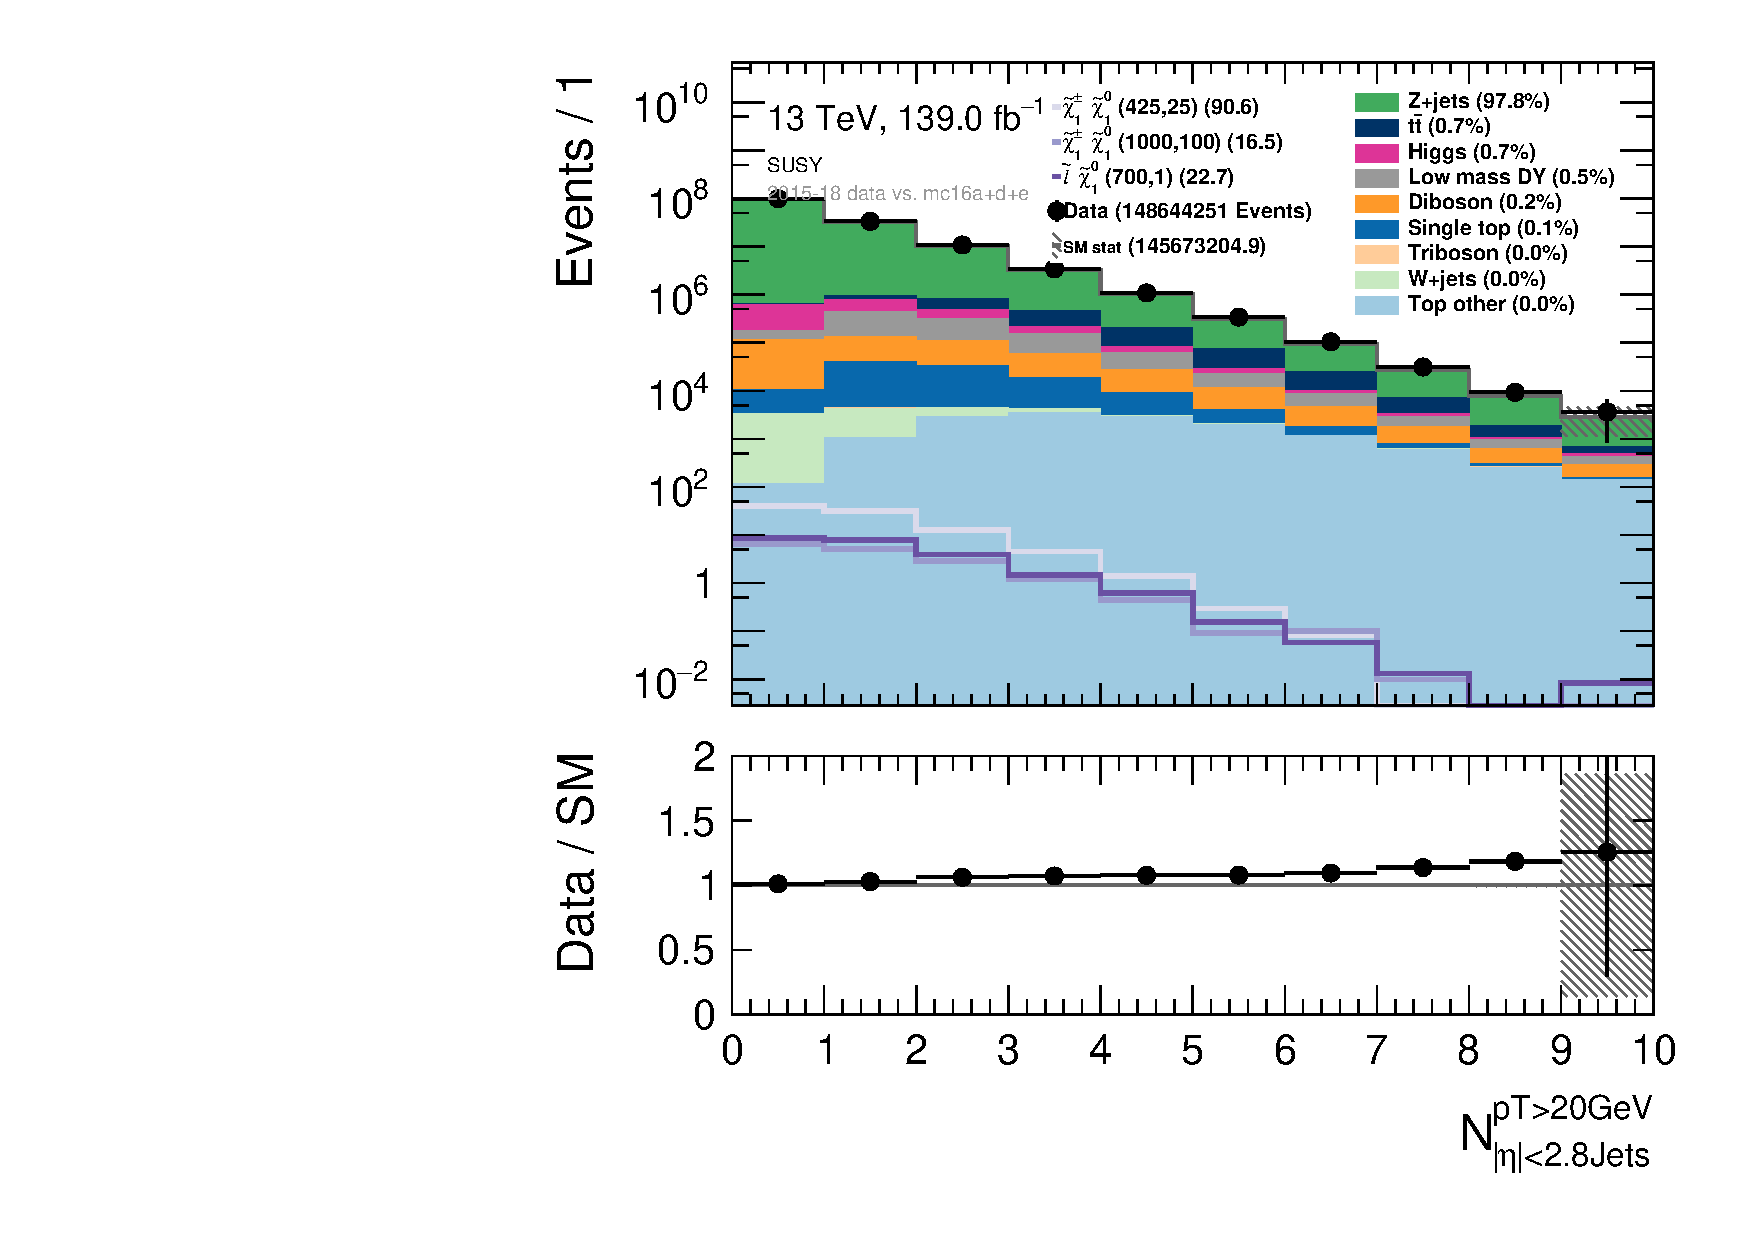
\includegraphics[width=\textwidth]{Figures/SUSYcuts/hist1d_nJet20_SUSY.pdf}
    \caption{Stransverse mass for direct slepton production.}
    \label{fig:my_label}
    \end{subfigure}
    \begin{subfigure}[t!]{0.49\textwidth}
        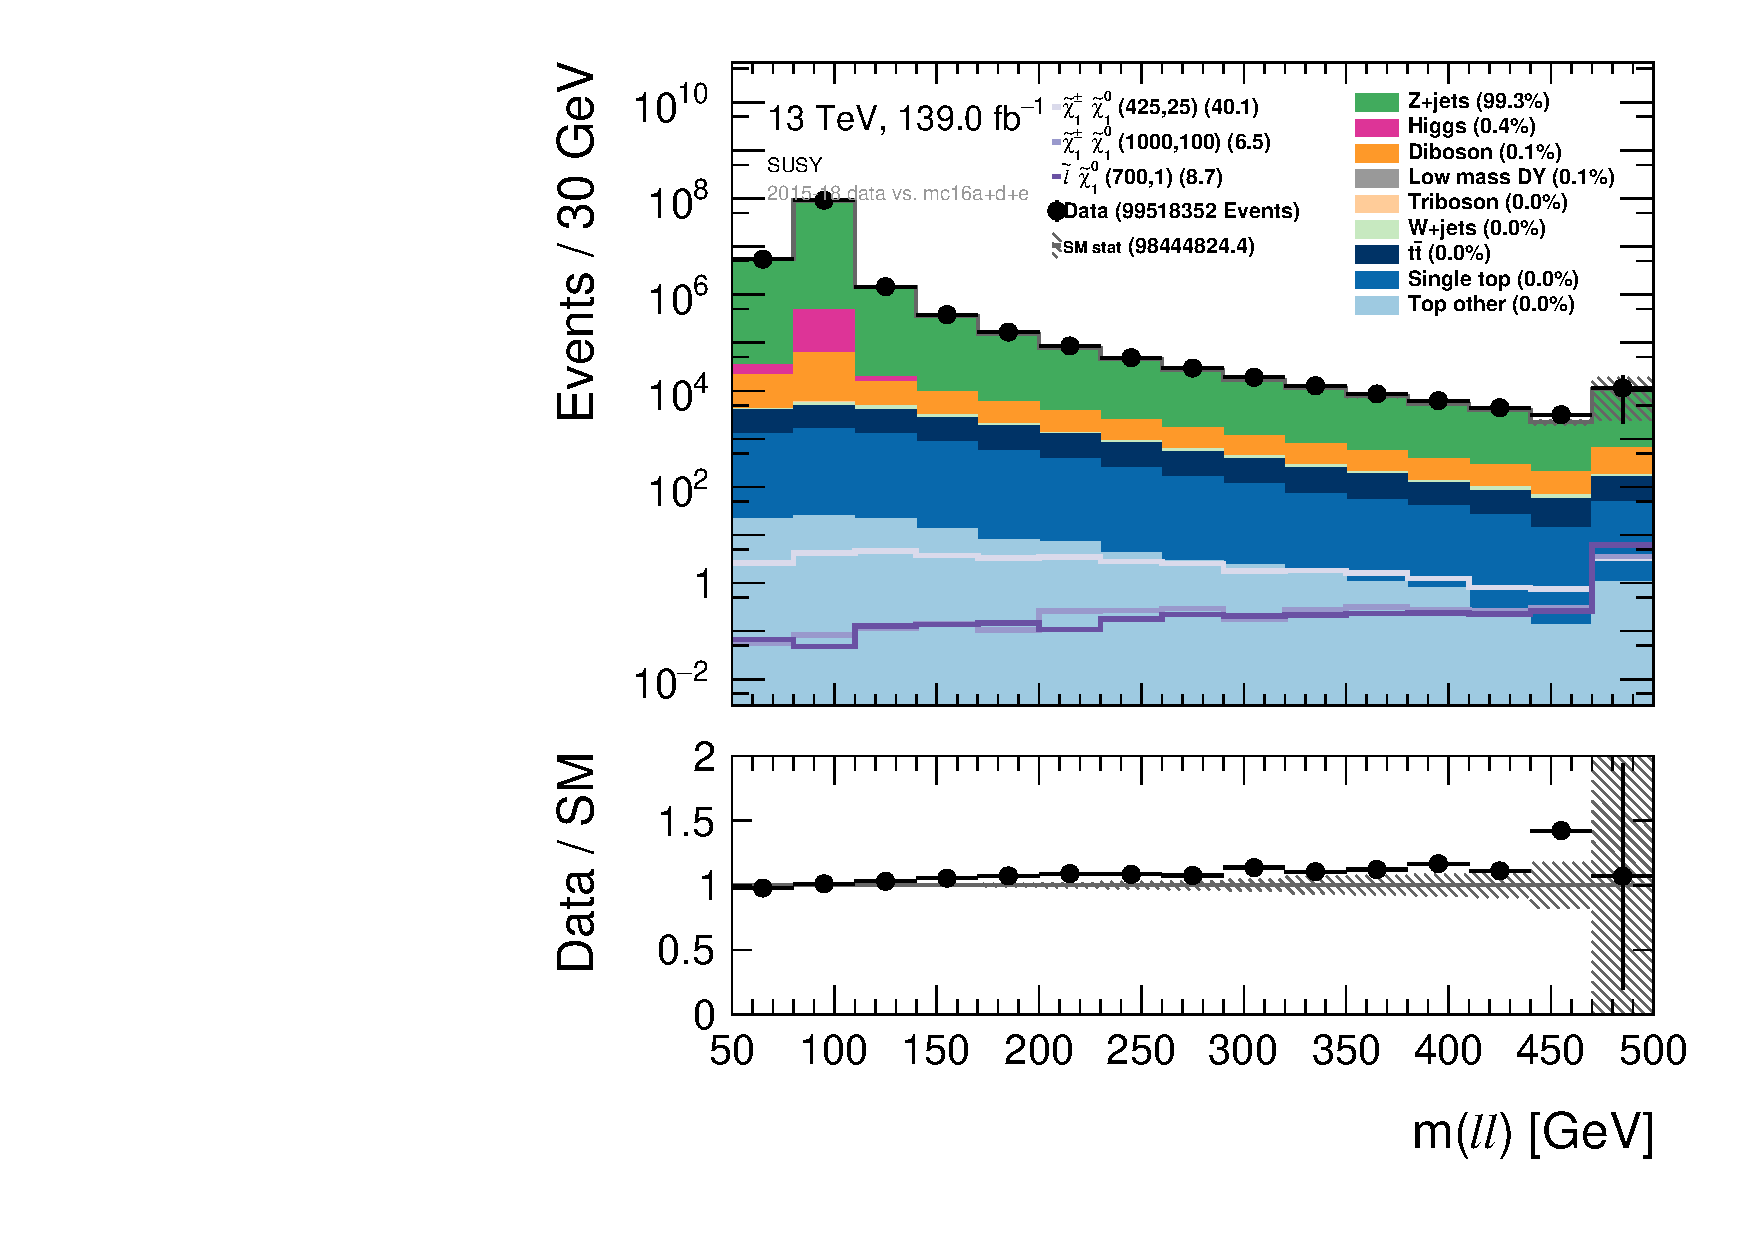
\includegraphics[width=\textwidth]{Figures/SUSYcuts/hist1d_mll_SUSY.pdf}
    \caption{Stransverse mass for chargino production via $\Tilde{l}/\Tilde{\nu}$.}
    \label{fig:my_label}
    \end{subfigure}
    \\
    \begin{subfigure}[t!]{0.49\textwidth}
        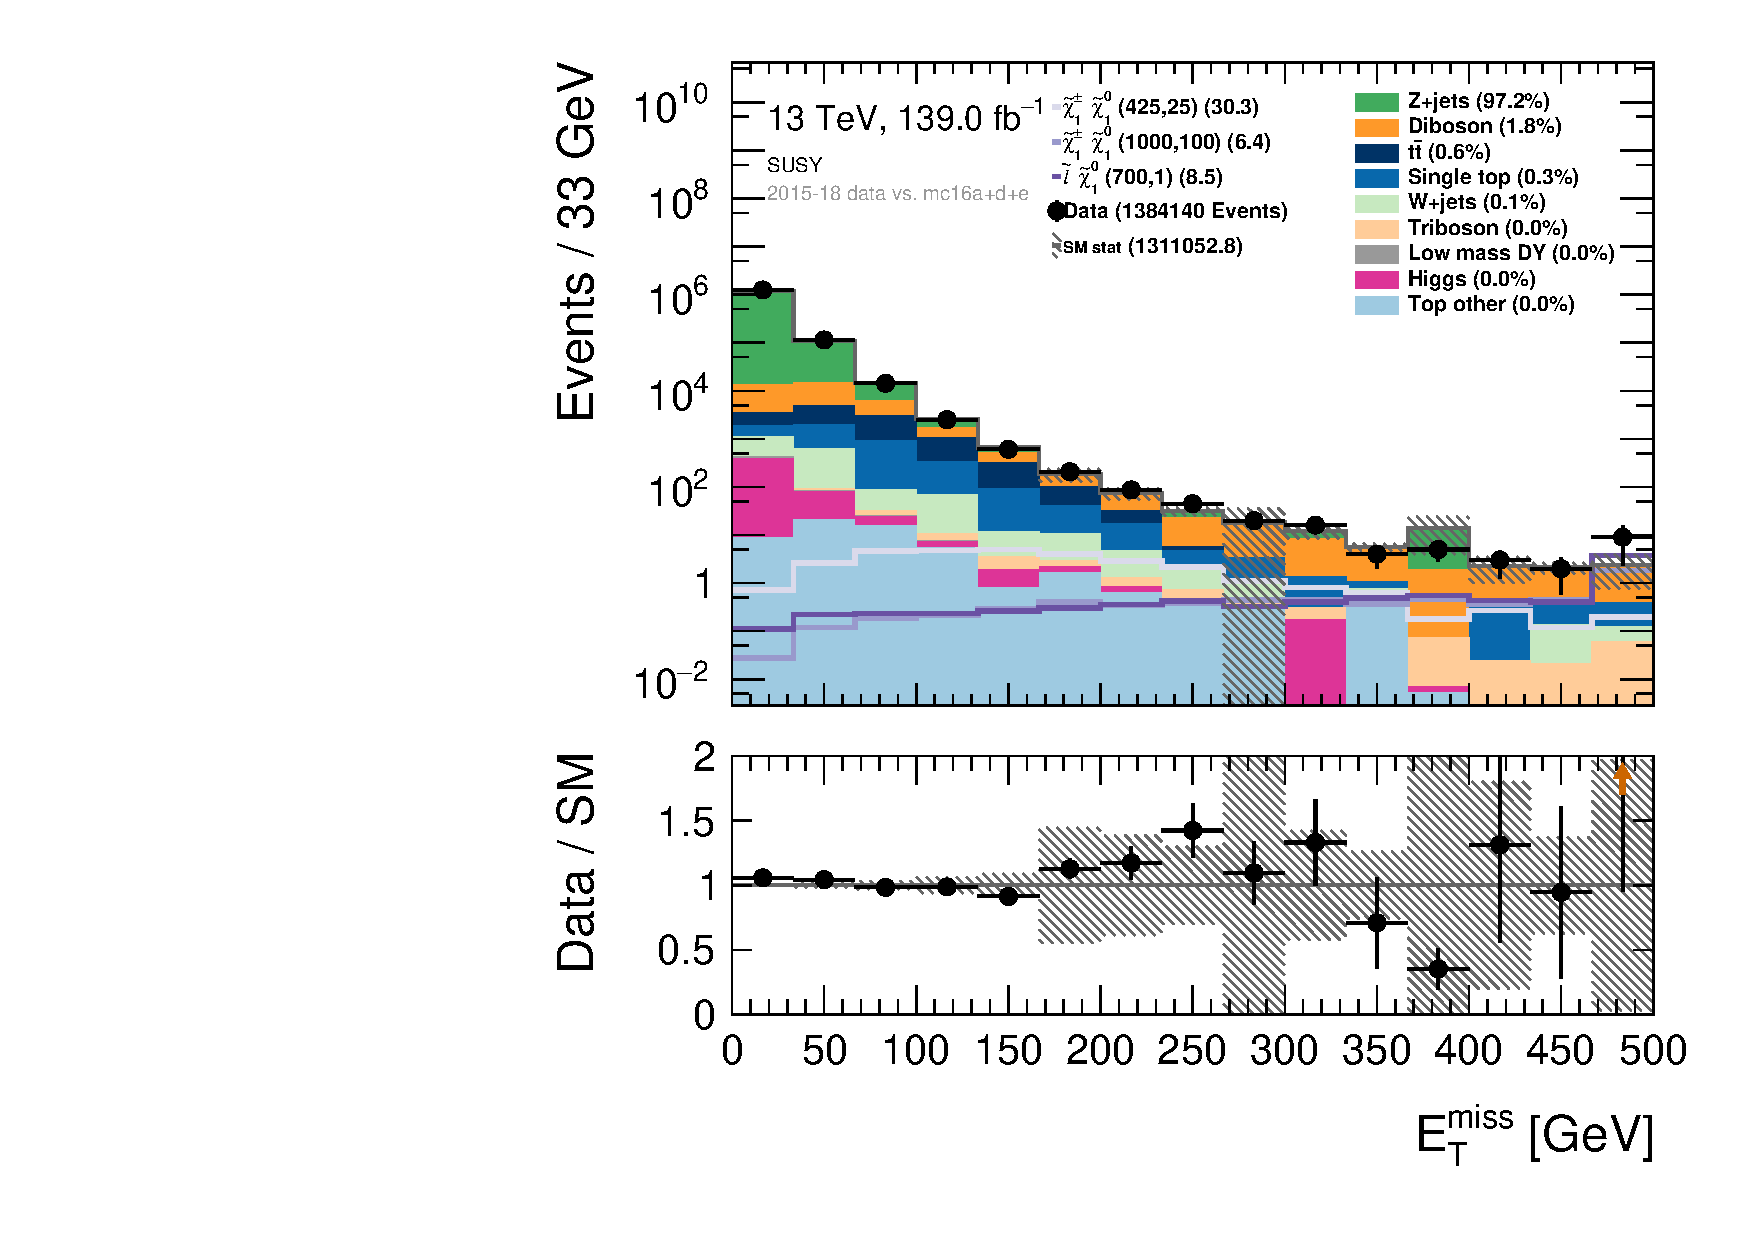
\includegraphics[width=\textwidth]{Figures/SUSYcuts/hist1d_met_Et_SUSY.pdf}
    \caption{Stransverse mass for chargino production via $W^\pm$.}
    \label{fig:my_label}
    \end{subfigure}
    \begin{subfigure}[t!]{0.49\textwidth}
        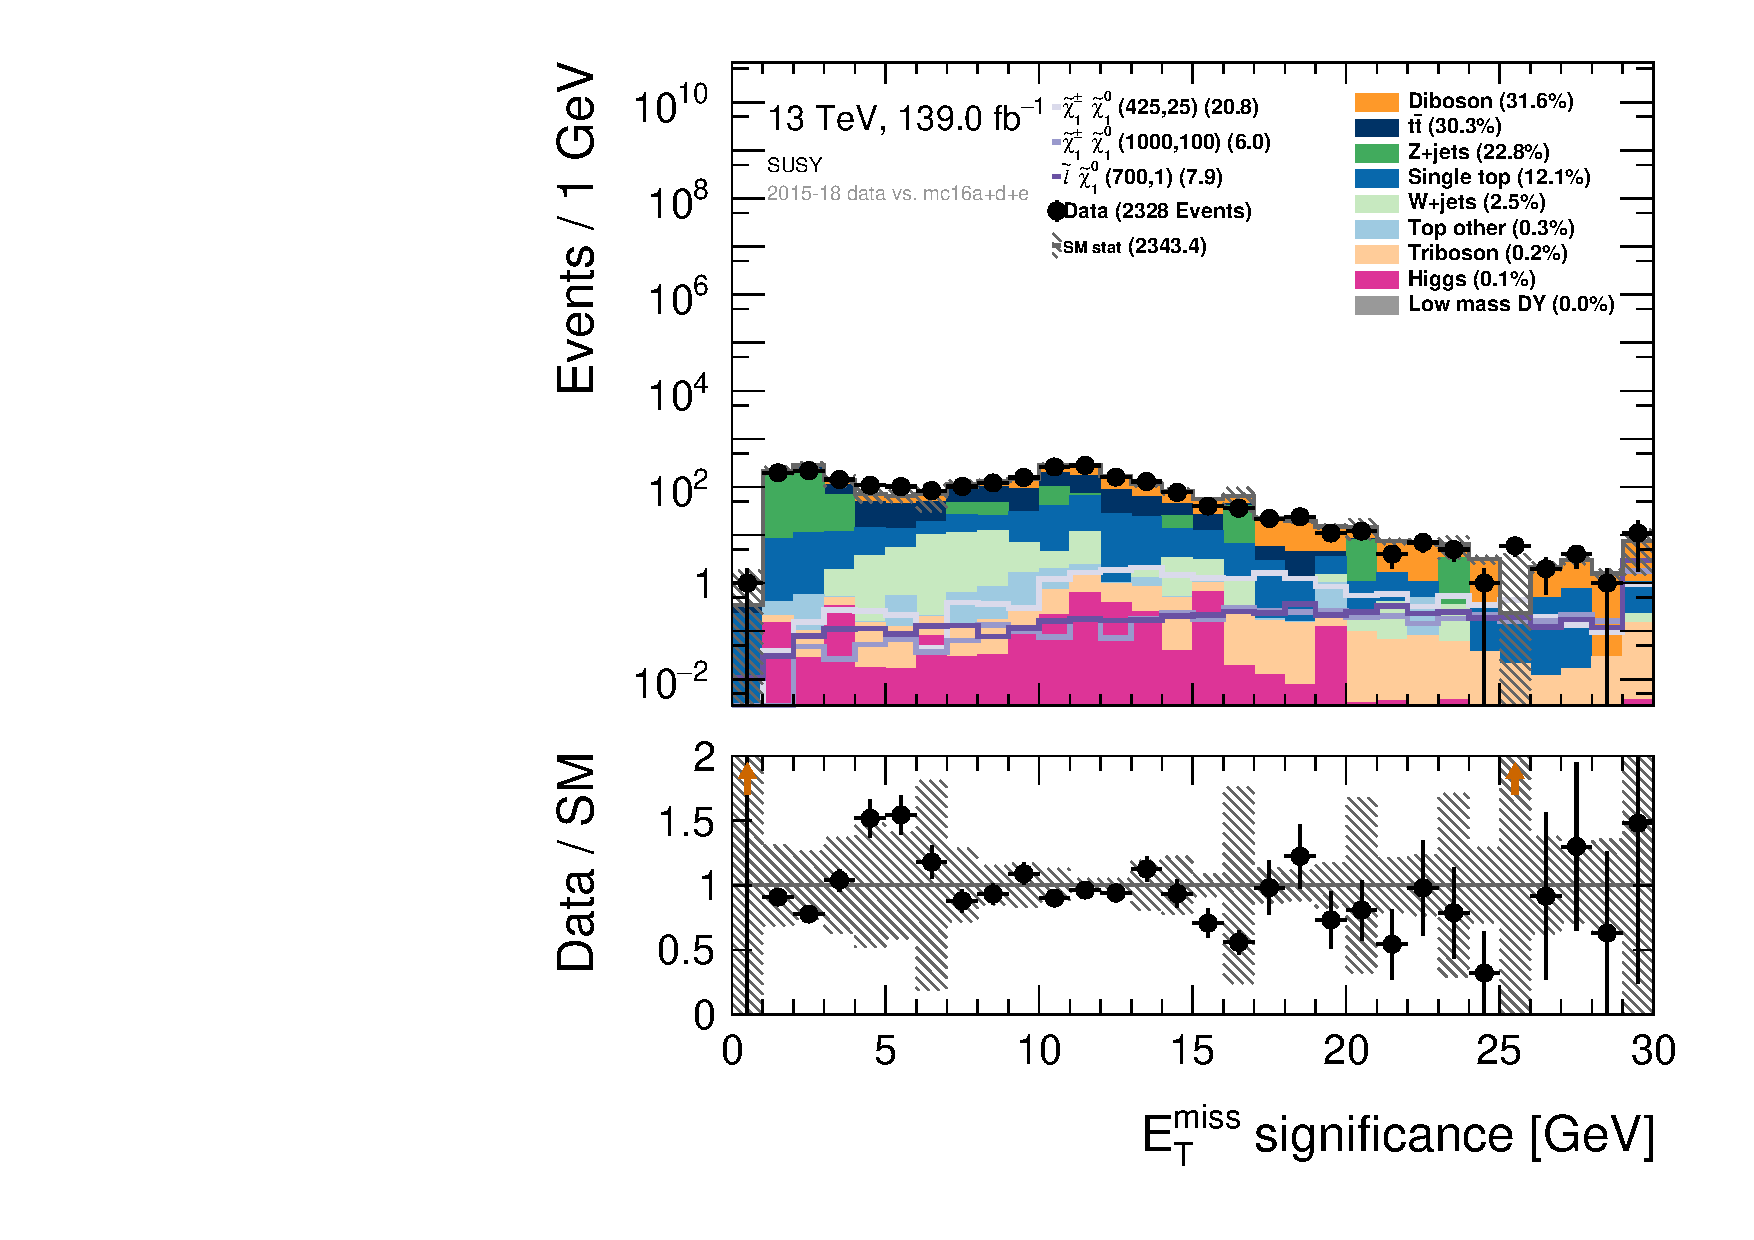
\includegraphics[width=\textwidth]{Figures/SUSYcuts/hist1d_met_Sign_SUSY.pdf}
    \caption{Missing transverse energy for mono-Z.}
    \label{fig:my_label}
    \end{subfigure}
    \\
    \begin{subfigure}[t!]{0.49\textwidth}
        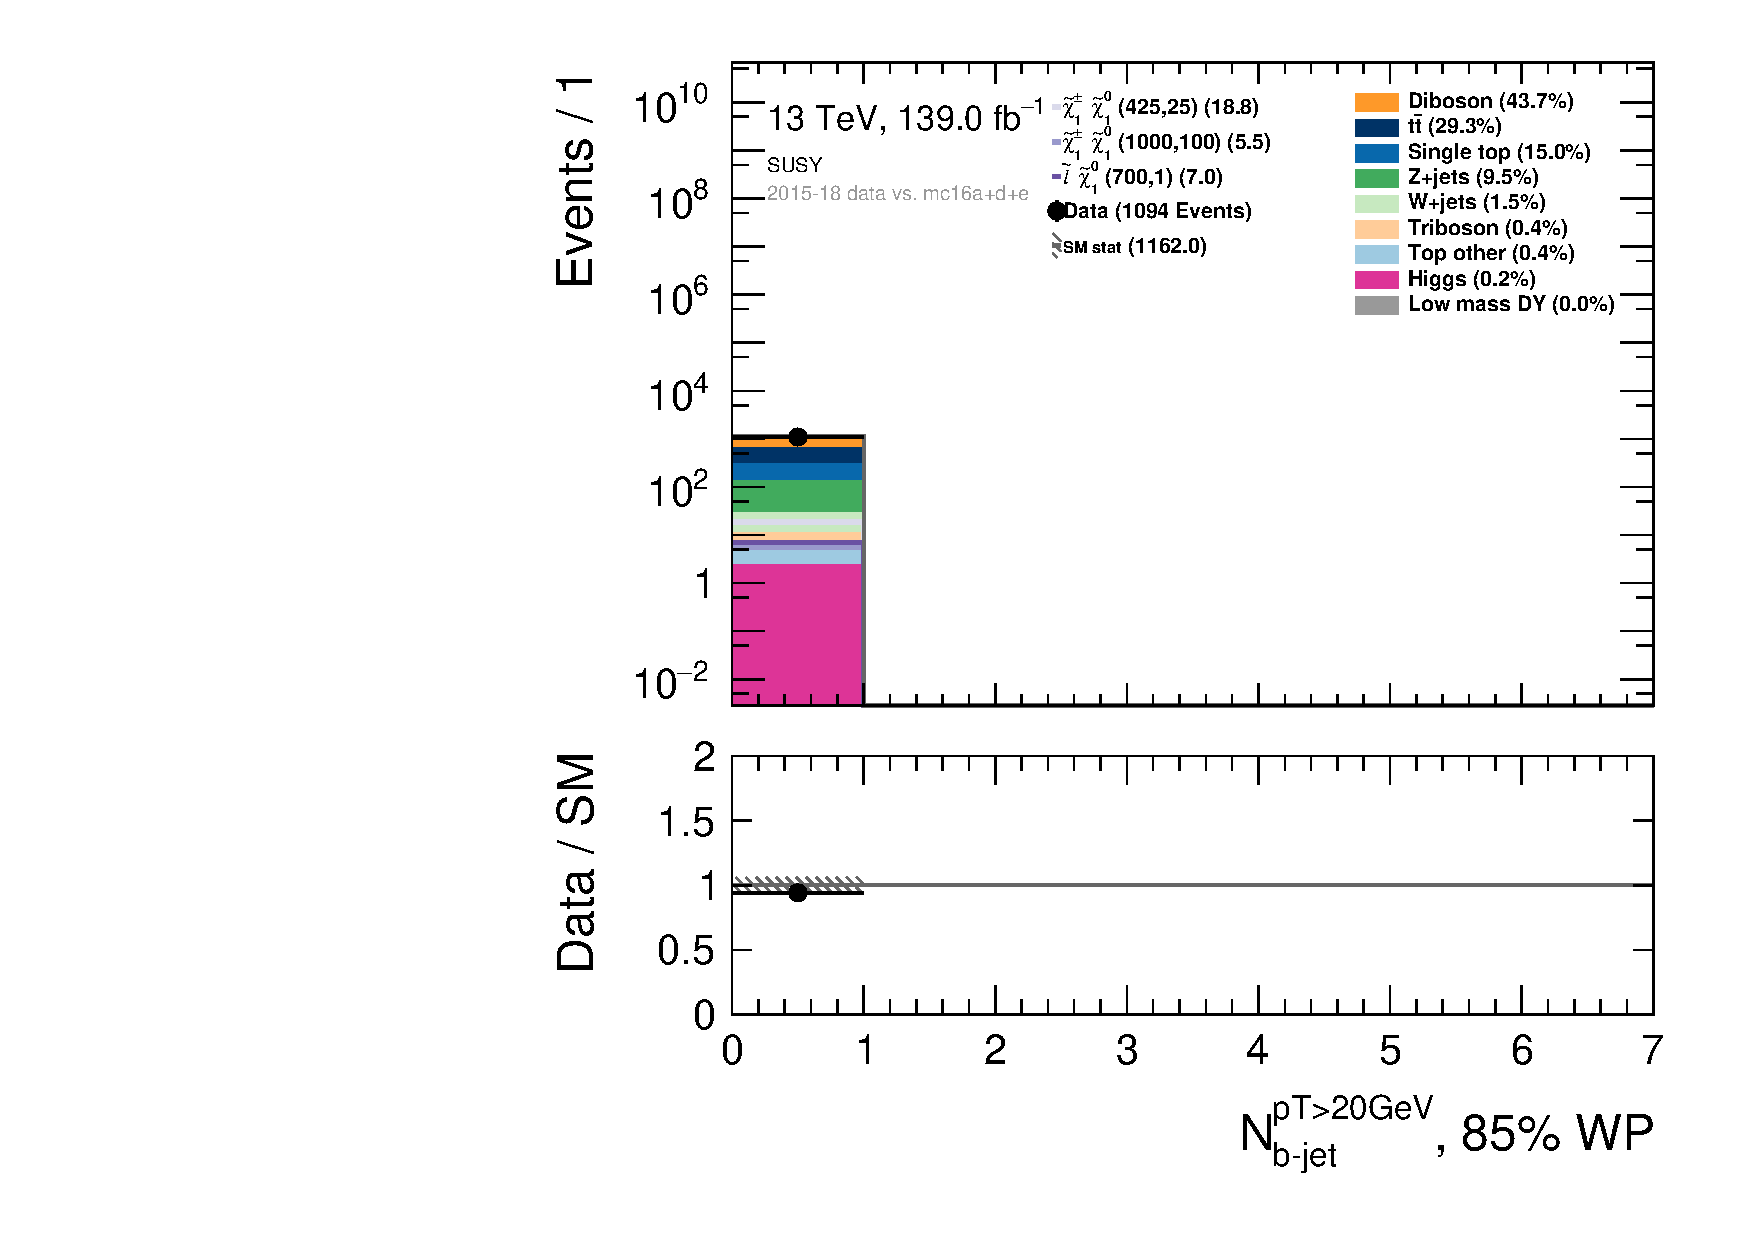
\includegraphics[width=\textwidth]{Figures/SUSYcuts/hist1d_nBJet20_MV2c10_FixedCutBEff_85_SUSY.pdf}
    \caption{Stransverse mass for chargino production via $W^\pm$.}
    \label{fig:my_label}
    \end{subfigure}
    \begin{subfigure}[t!]{0.49\textwidth}
        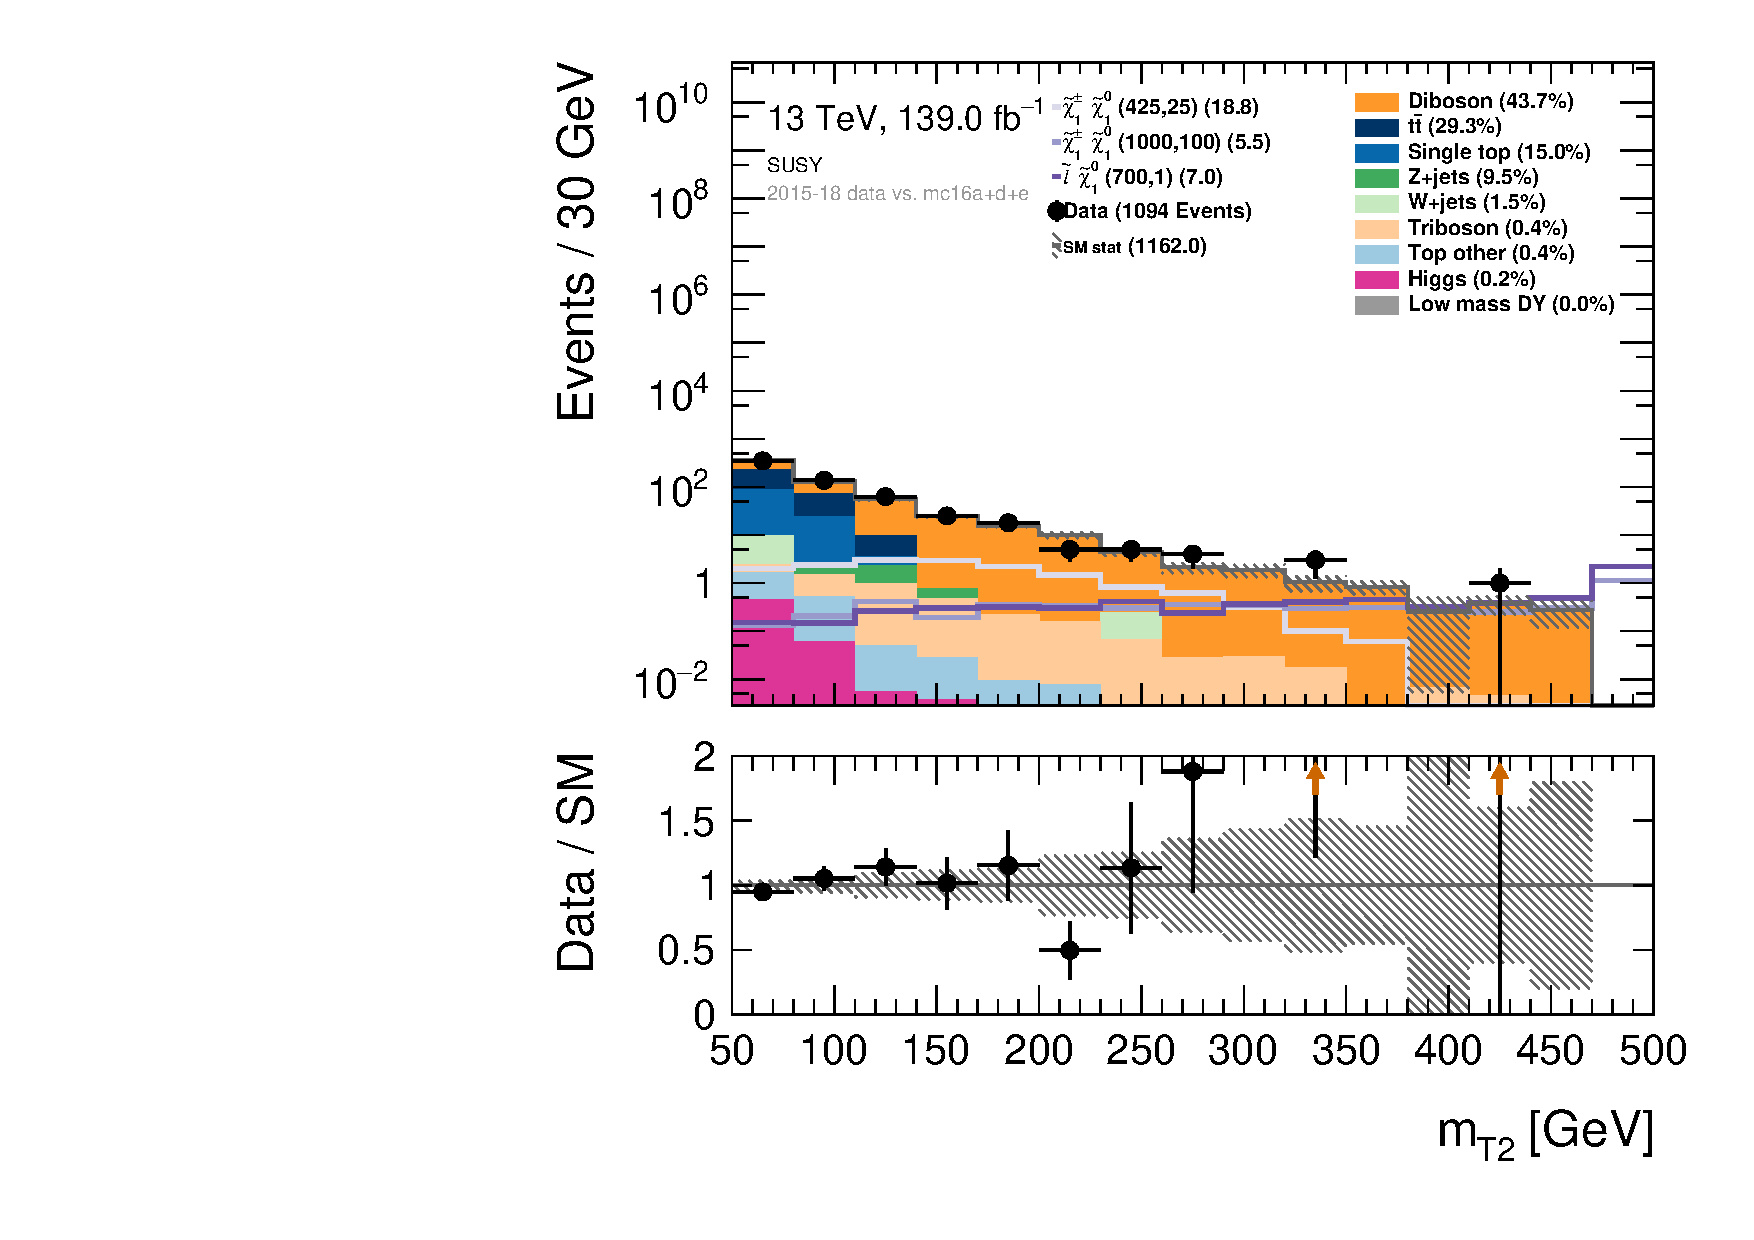
\includegraphics[width=\textwidth]{Figures/SUSYcuts/hist1d_mt2_SUSY.pdf}
    \caption{Missing transverse energy for mono-Z.}
    \label{fig:my_label}
    \end{subfigure}
    \caption{Plot of the four most important variables in direct slepton production with a cut on only two leptons with opposite charge in the final state.}
    \label{fig:cutandcountStepsSUSY}
\end{figure}
\restoregeometry



















\newgeometry{twoside,inner=3cm,outer=2cm}
\begin{figure}[H]
%\begin{minipage}{2\textwidth}
%\begin{adjustwidth}{-3cm}{-3cm}
\centering
%\advance\leftskip-4cm 
%\advance\rightskip-4cm 
    \begin{subfigure}[t!]{0.49\textwidth}
        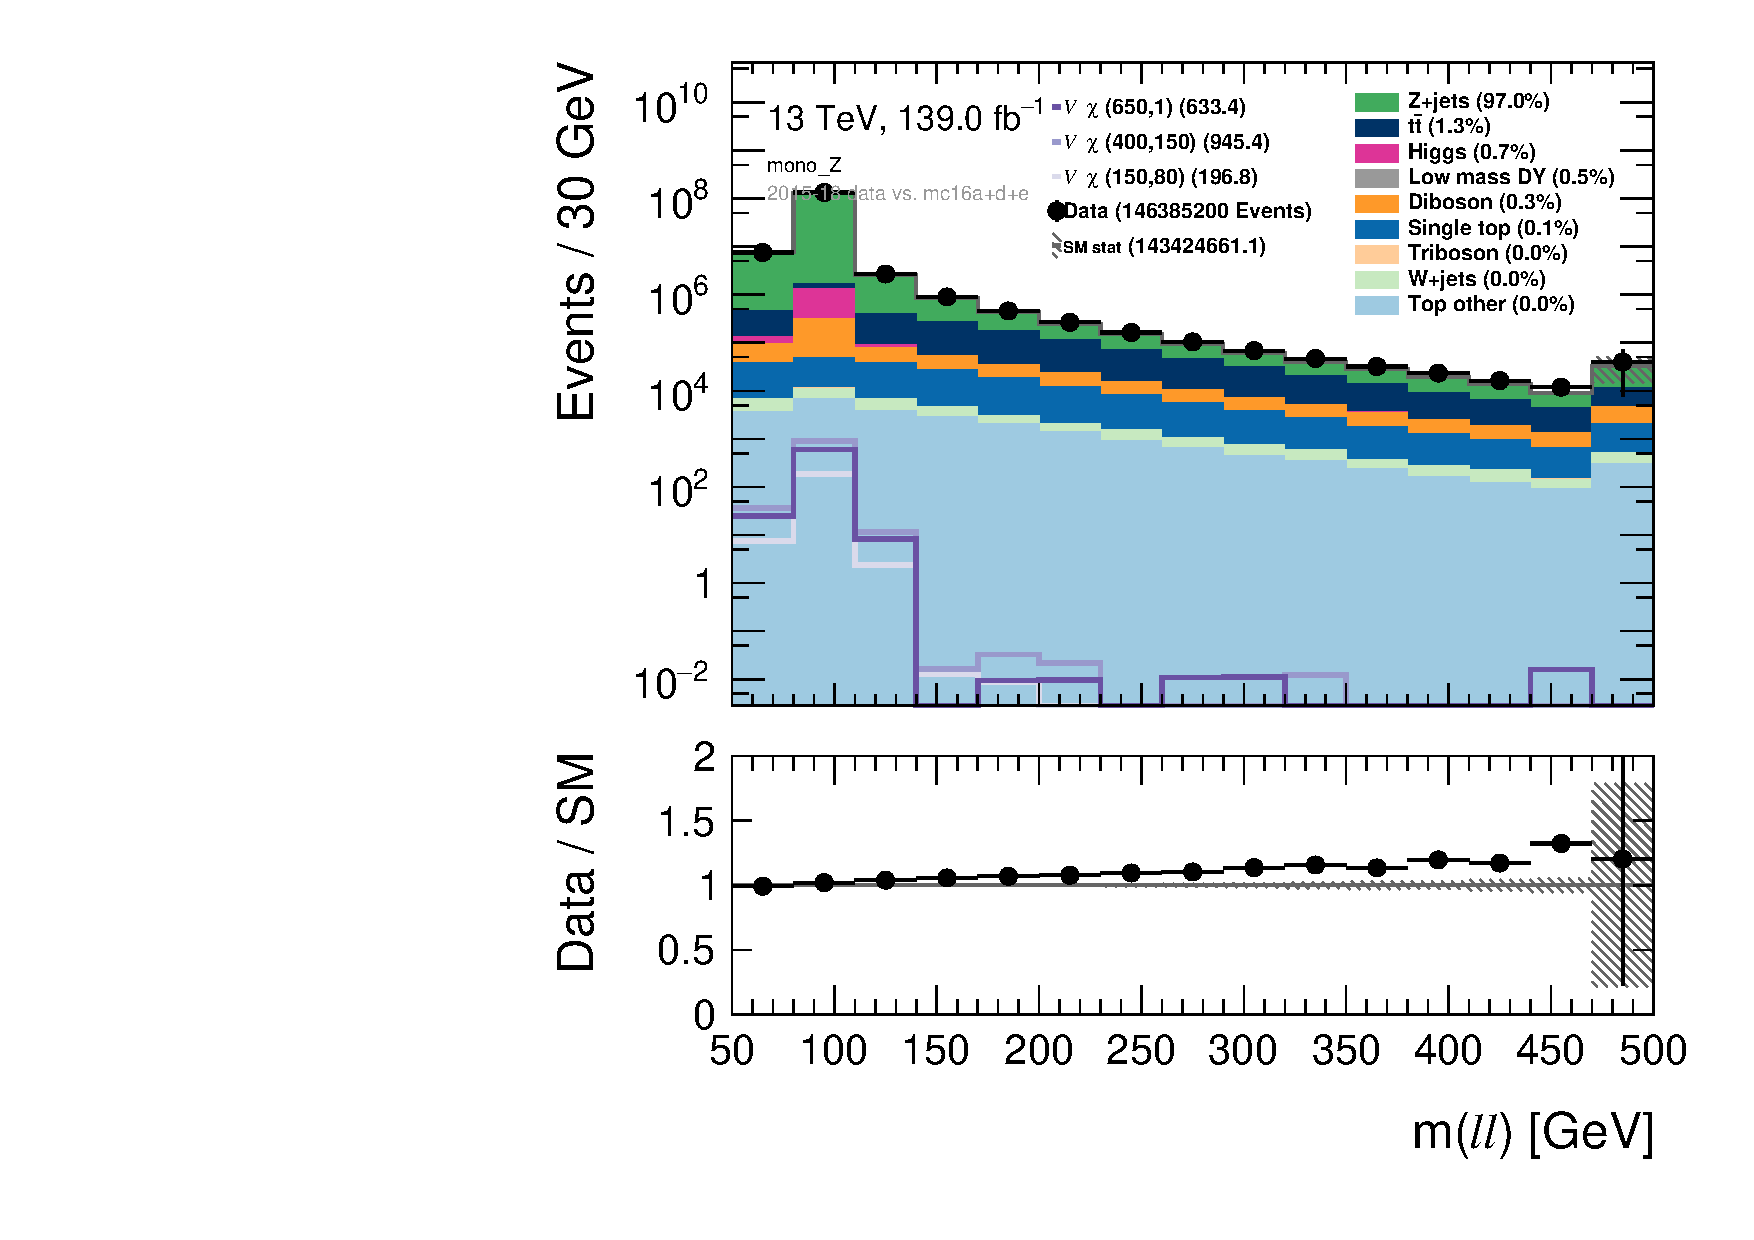
\includegraphics[width=\textwidth]{Figures/MonoZcuts/hist1d_mll_mono_Z.pdf}
    \caption{Stransverse mass for direct slepton production.}
    \label{fig:my_label}
    \end{subfigure}
    \begin{subfigure}[t!]{0.49\textwidth}
        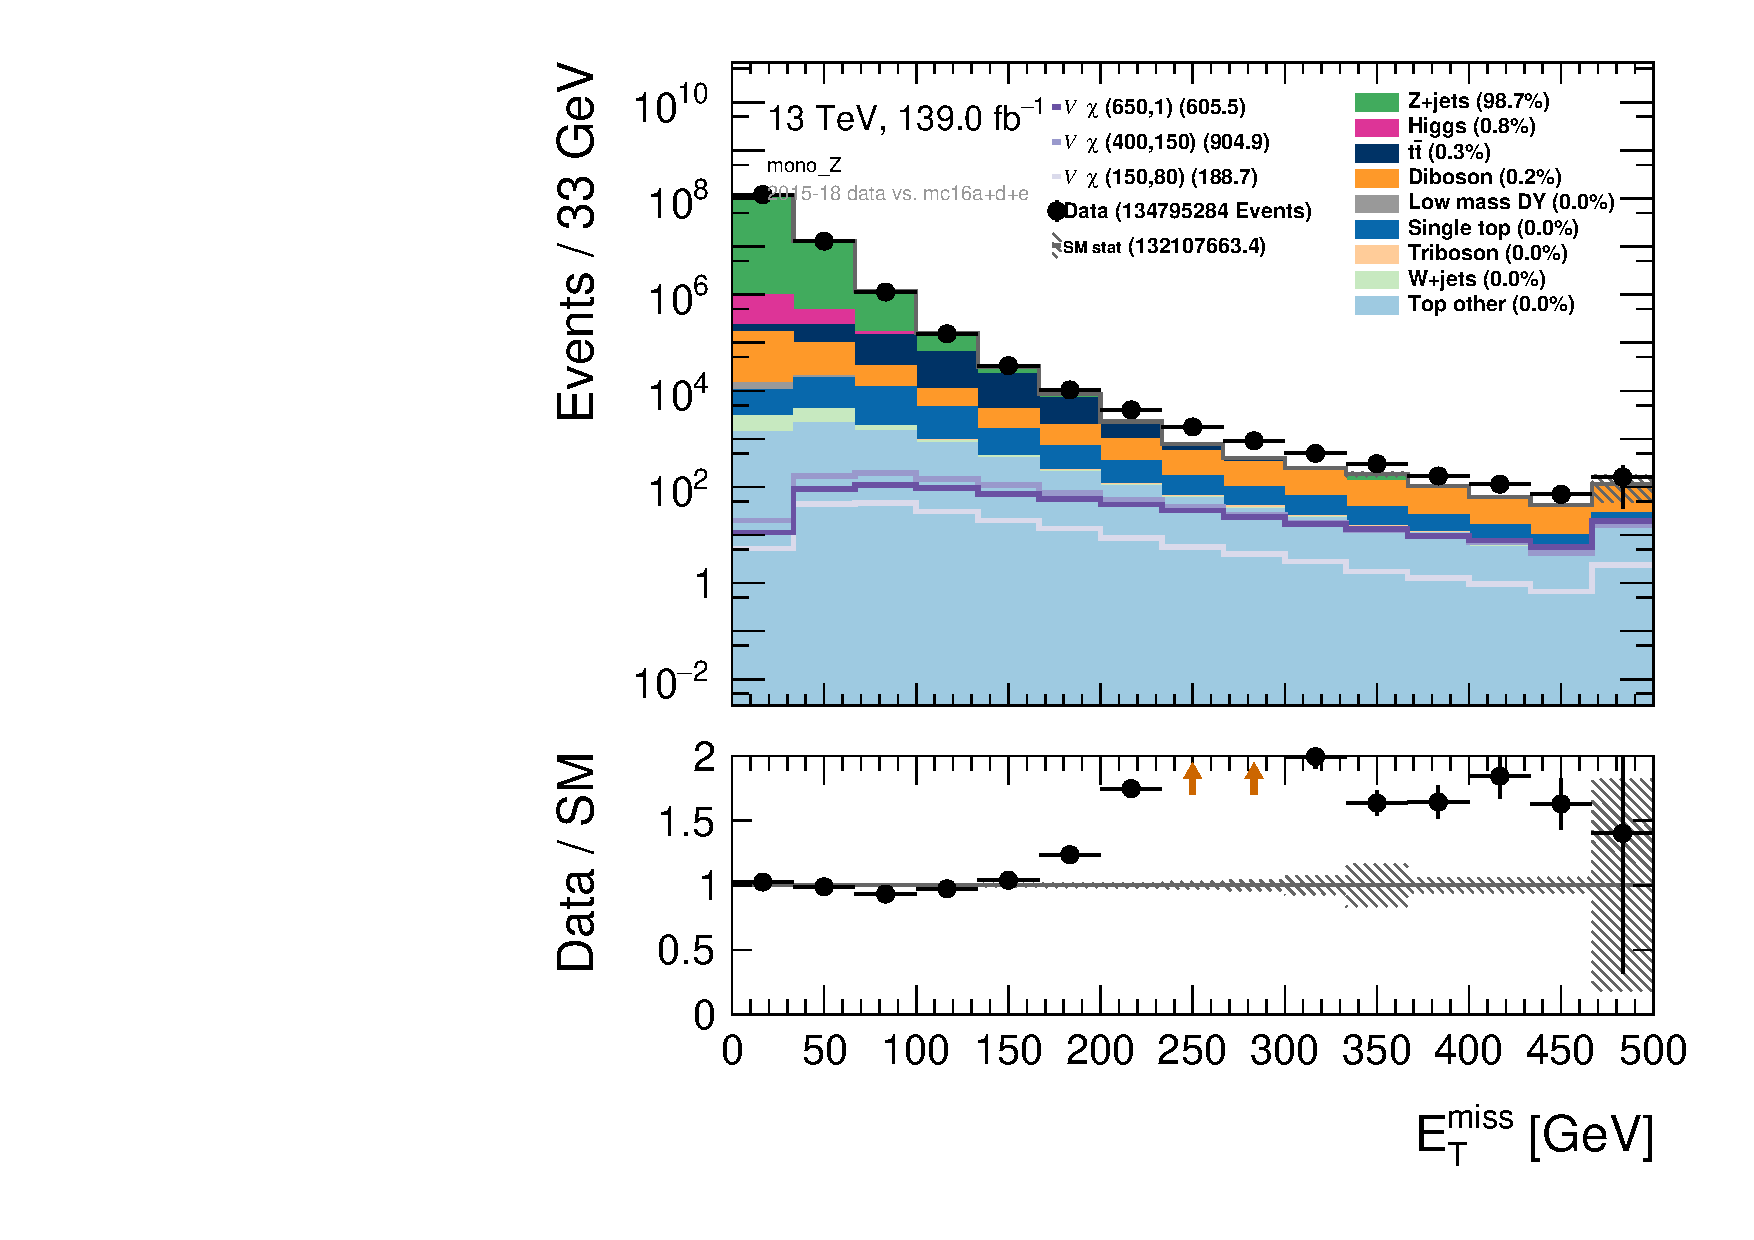
\includegraphics[width=\textwidth]{Figures/MonoZcuts/hist1d_met_Et_mono_Z_1.pdf}
    \caption{Stransverse mass for chargino production via $\Tilde{l}/\Tilde{\nu}$.}
    \label{fig:my_label}
    \end{subfigure}
    \\
    \begin{subfigure}[t!]{0.49\textwidth}
        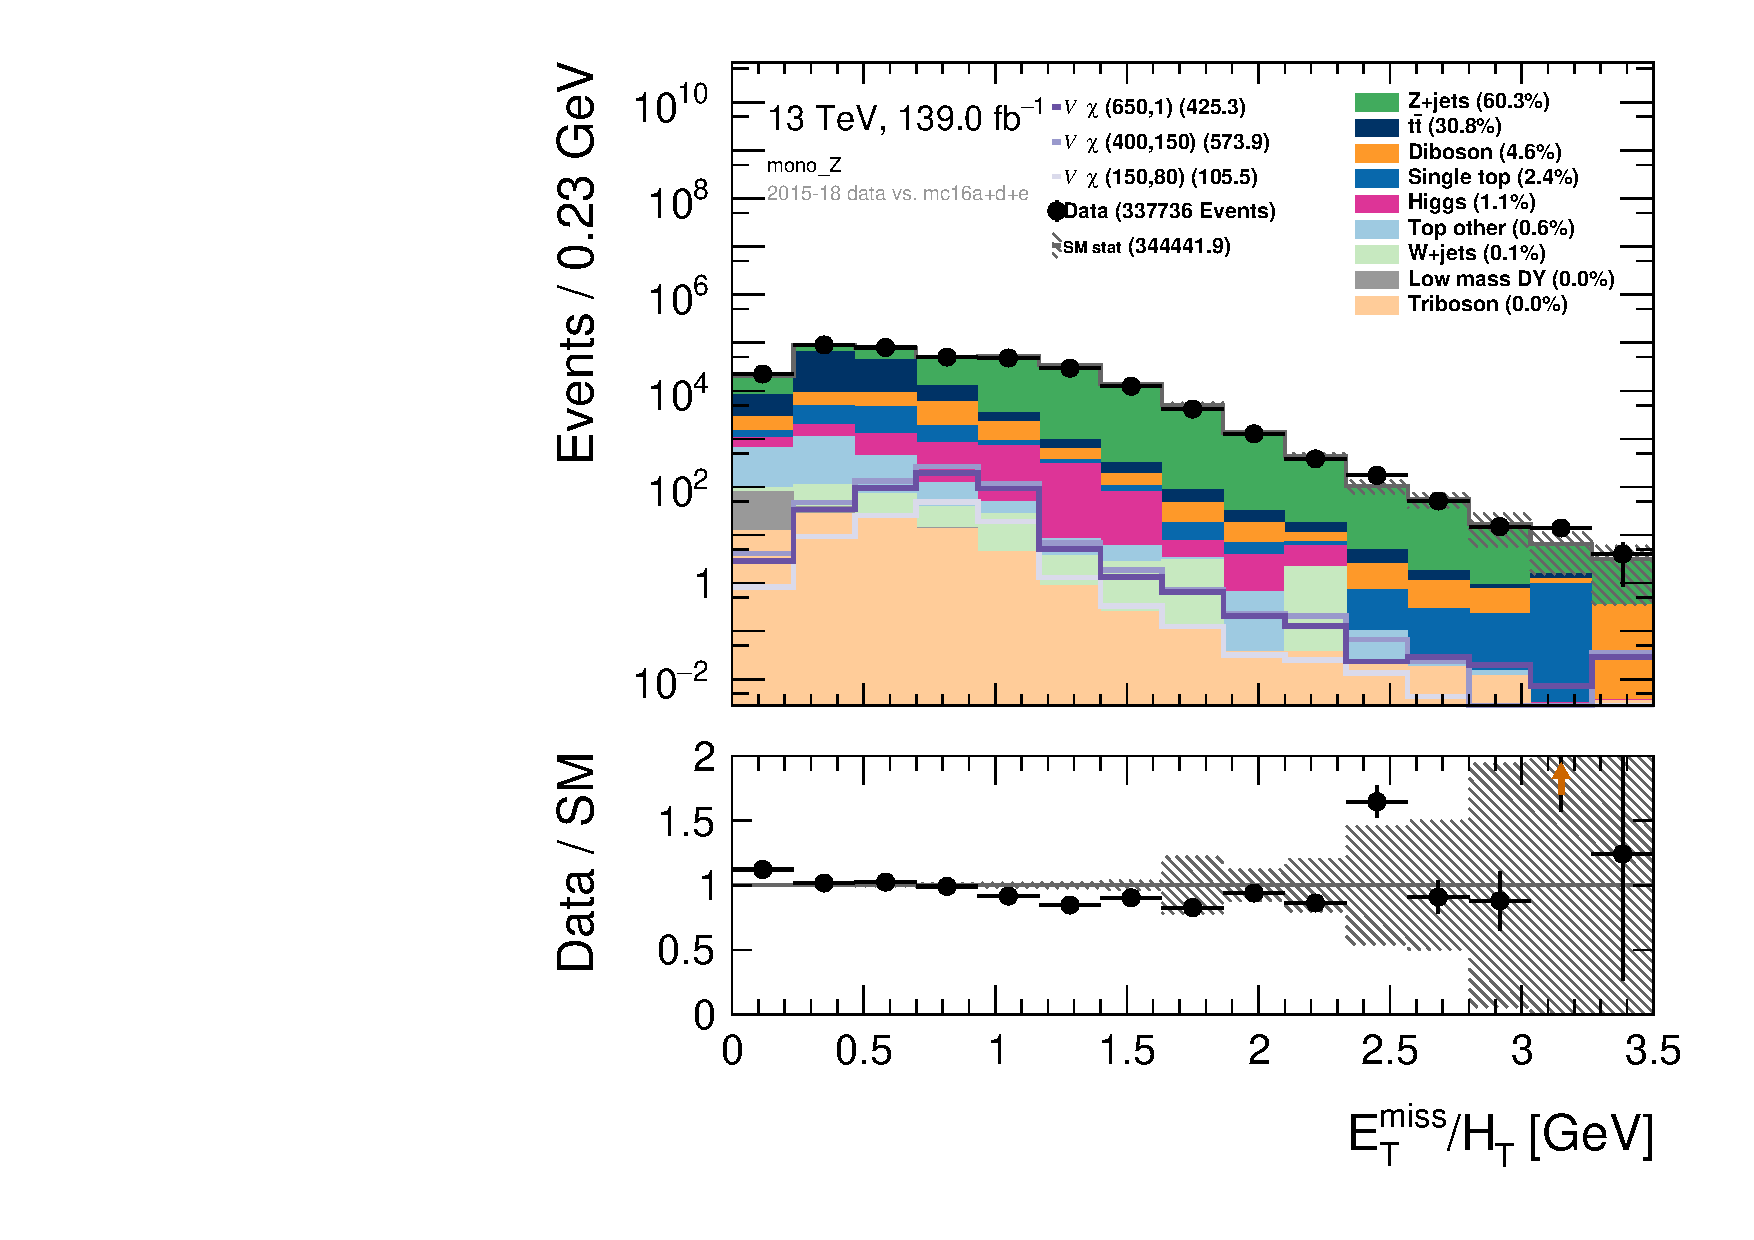
\includegraphics[width=\textwidth]{Figures/MonoZcuts/hist1d_met_HT_mono_Z.pdf}
    \caption{Stransverse mass for chargino production via $W^\pm$.}
    \label{fig:my_label}
    \end{subfigure}
    \begin{subfigure}[t!]{0.49\textwidth}
        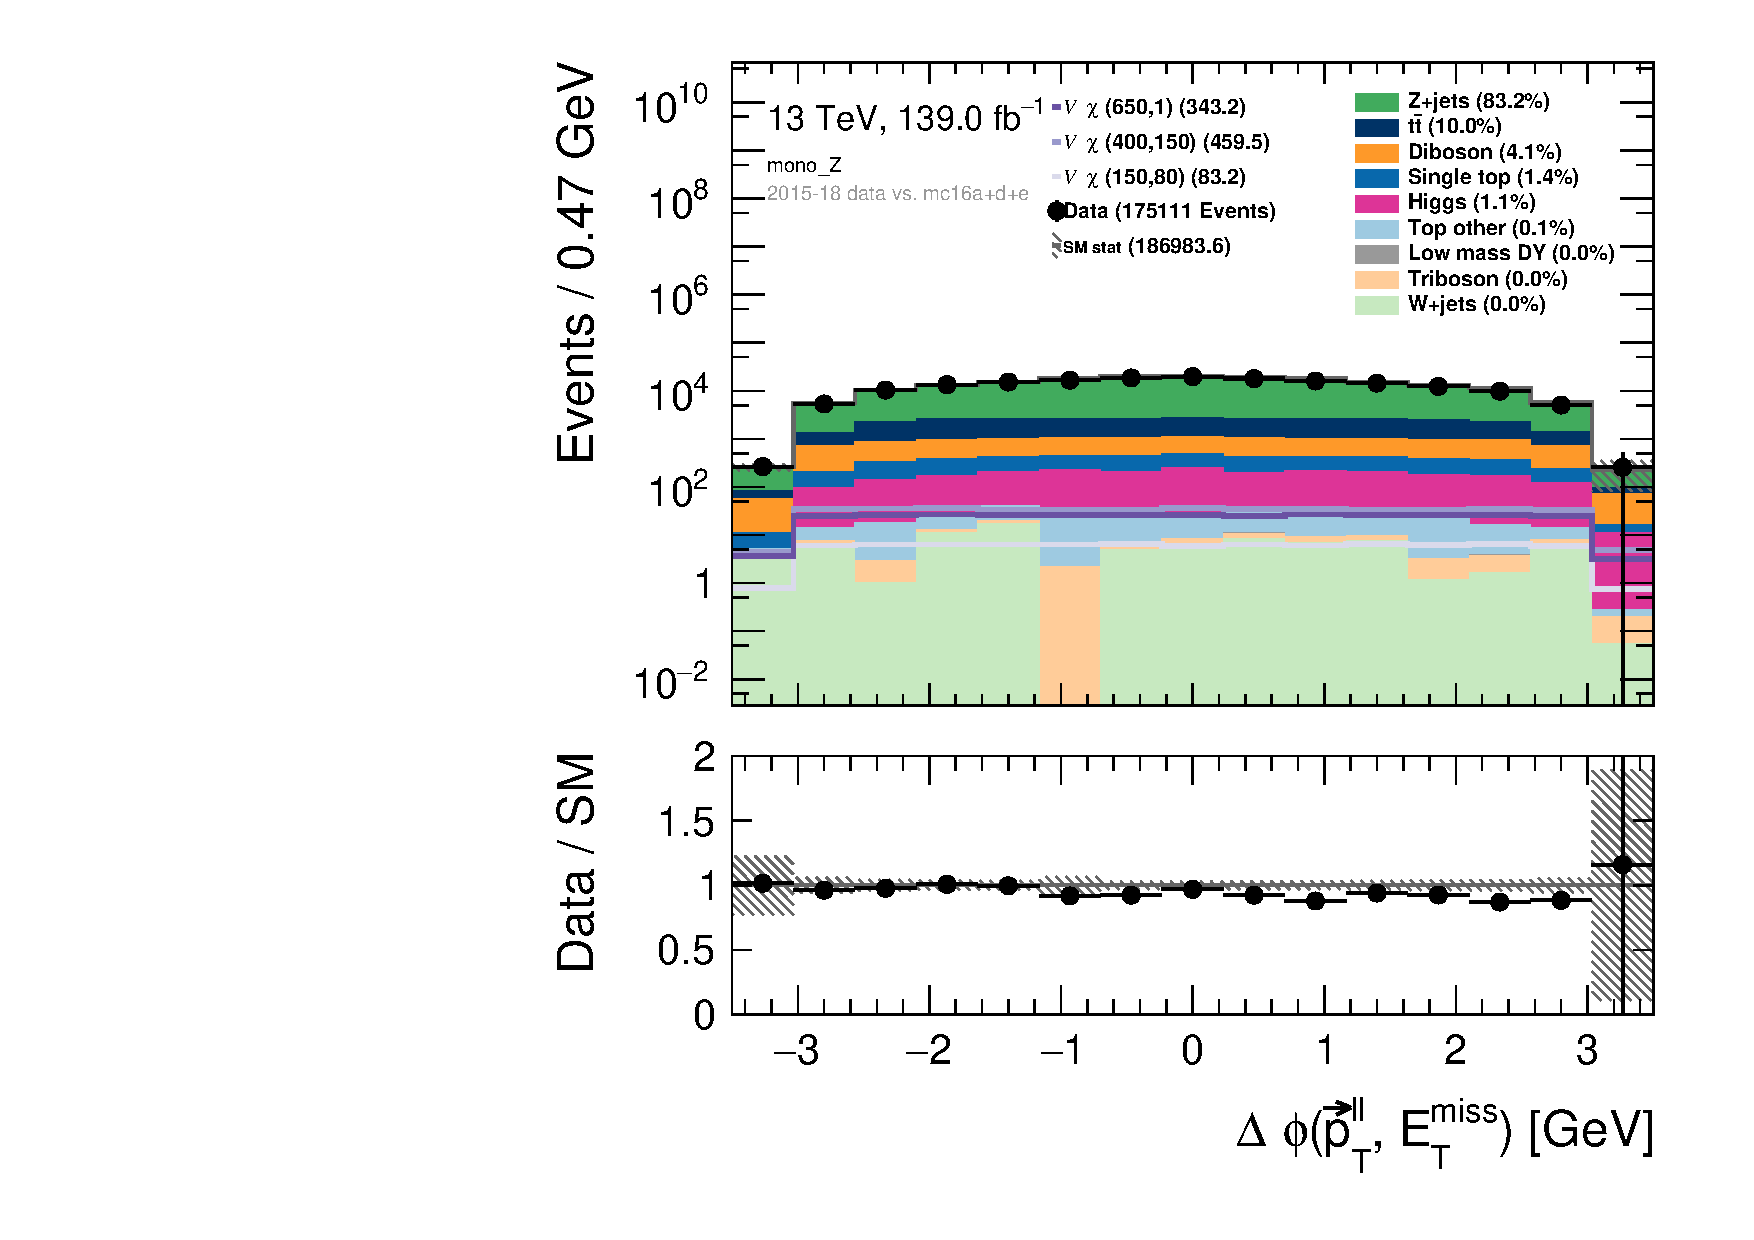
\includegraphics[width=\textwidth]{Figures/MonoZcuts/hist1d_deltaPhi_mono_Z.pdf}
    \caption{Missing transverse energy for mono-Z.}
    \label{fig:my_label}
    \end{subfigure}
    \\
    \begin{subfigure}[t!]{0.49\textwidth}
        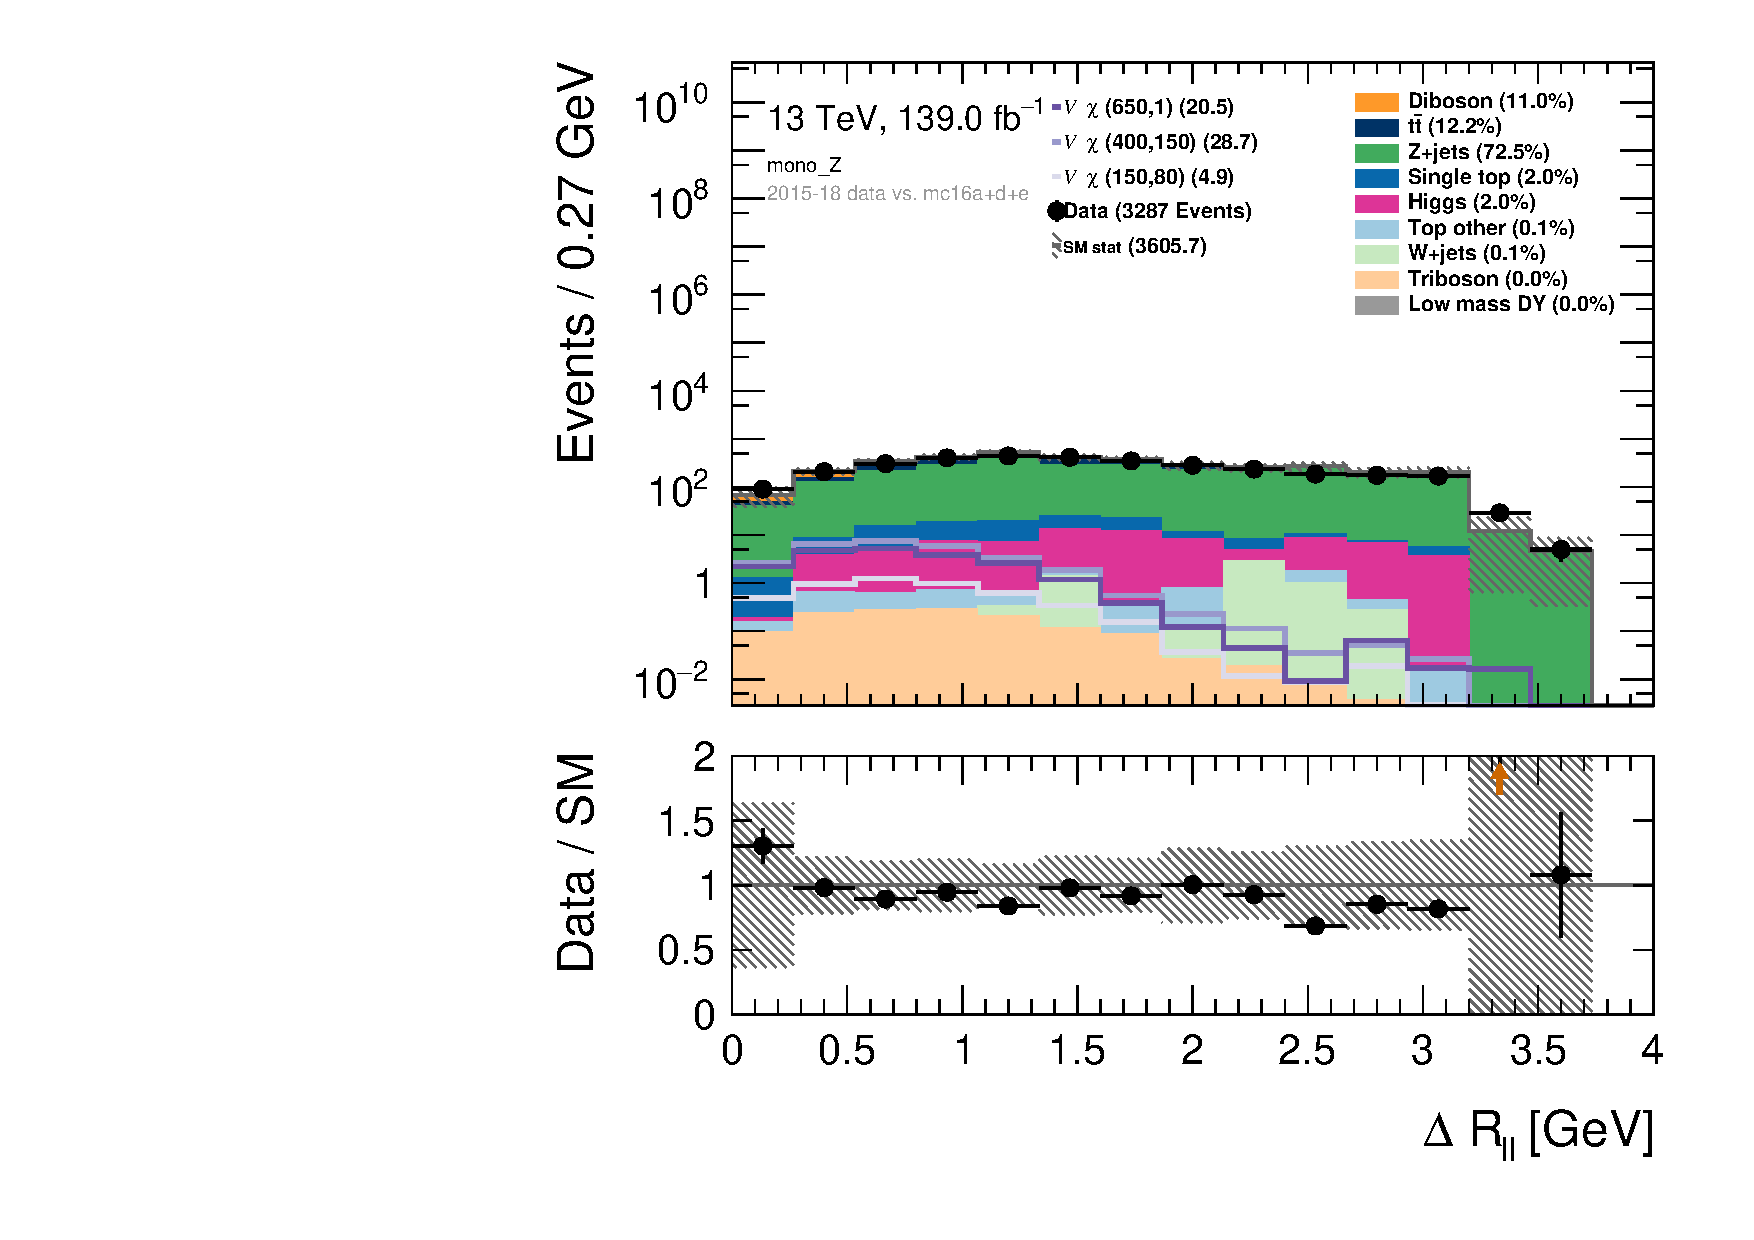
\includegraphics[width=\textwidth]{Figures/MonoZcuts/hist1d_deltaRll_mono_Z.pdf}
    \caption{Stransverse mass for chargino production via $W^\pm$.}
    \label{fig:my_label}
    \end{subfigure}
    \begin{subfigure}[t!]{0.49\textwidth}
        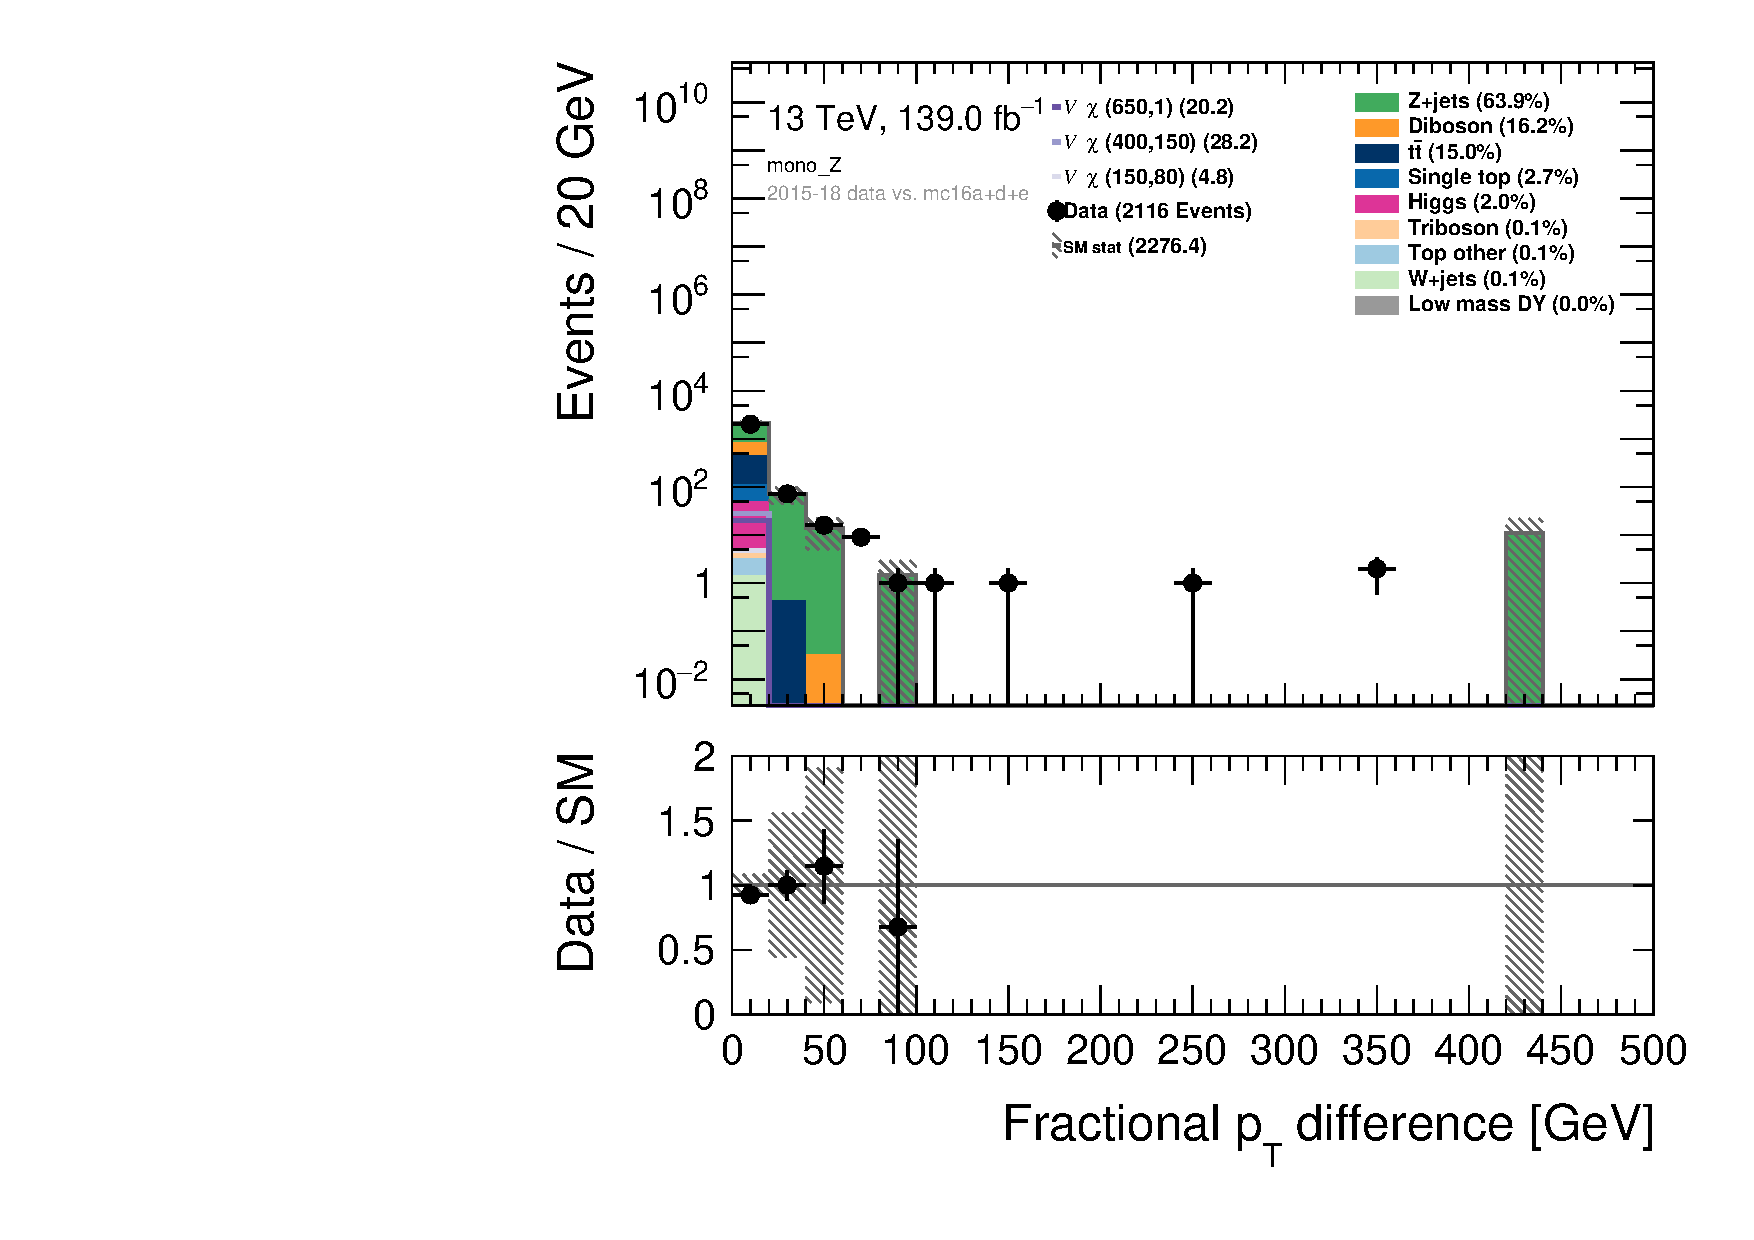
\includegraphics[width=\textwidth]{Figures/MonoZcuts/hist1d_pTdiff_mono_Z.pdf}
    \caption{Missing transverse energy for mono-Z.}
    \label{fig:my_label}
    \end{subfigure}
\end{figure}
\restoregeometry


\newgeometry{twoside,inner=3cm,outer=2cm}
\begin{figure}[H] \ContinuedFloat
%\begin{minipage}{2\textwidth}
%\begin{adjustwidth}{-3cm}{-3cm}
\centering
%\advance\leftskip-4cm 
%\advance\rightskip-4cm 
    \begin{subfigure}[t!]{0.49\textwidth}
        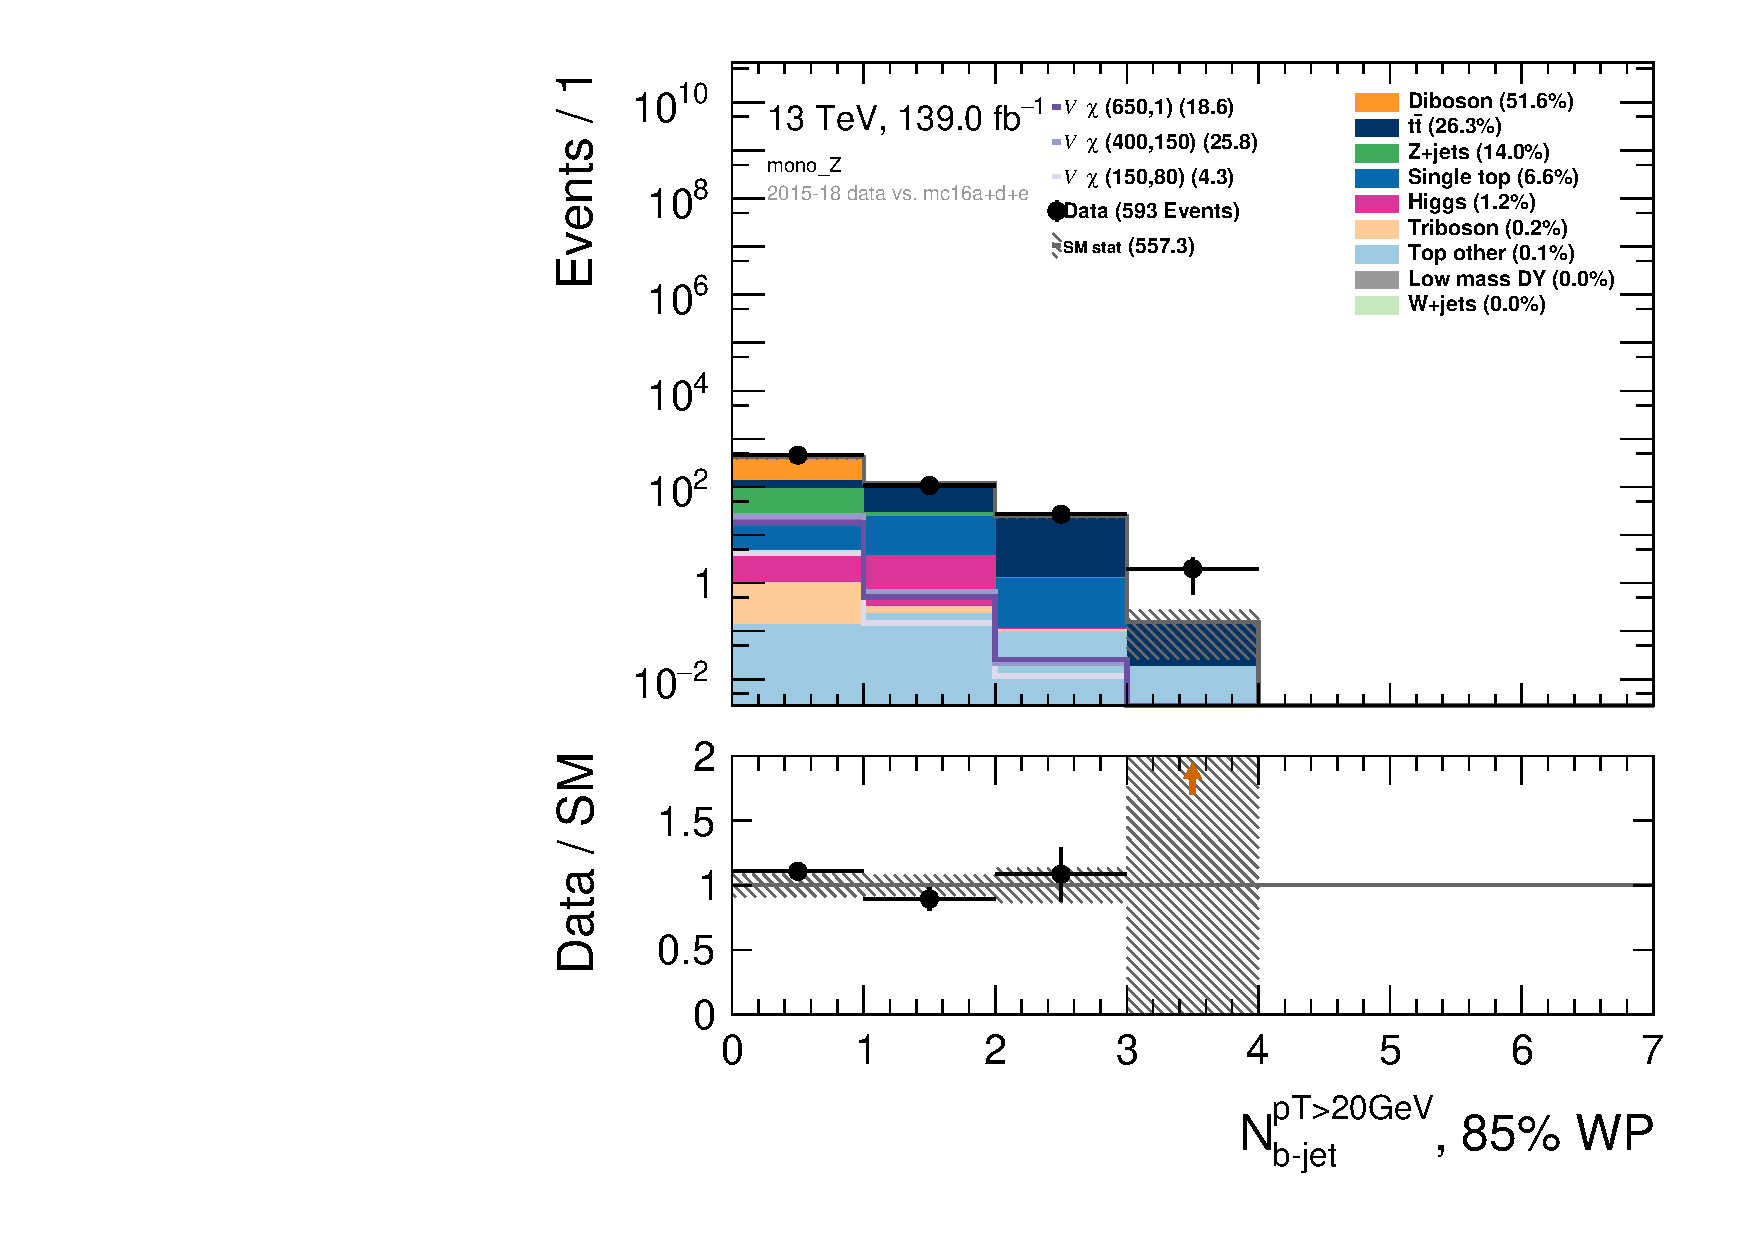
\includegraphics[width=\textwidth]{Figures/MonoZcuts/hist1d_nBJet20_MV2c10_FixedCutBEff_85_mono_Z.pdf}
    \caption{Stransverse mass for direct slepton production.}
    \label{fig:my_label}
    \end{subfigure}
    \begin{subfigure}[t!]{0.49\textwidth}
        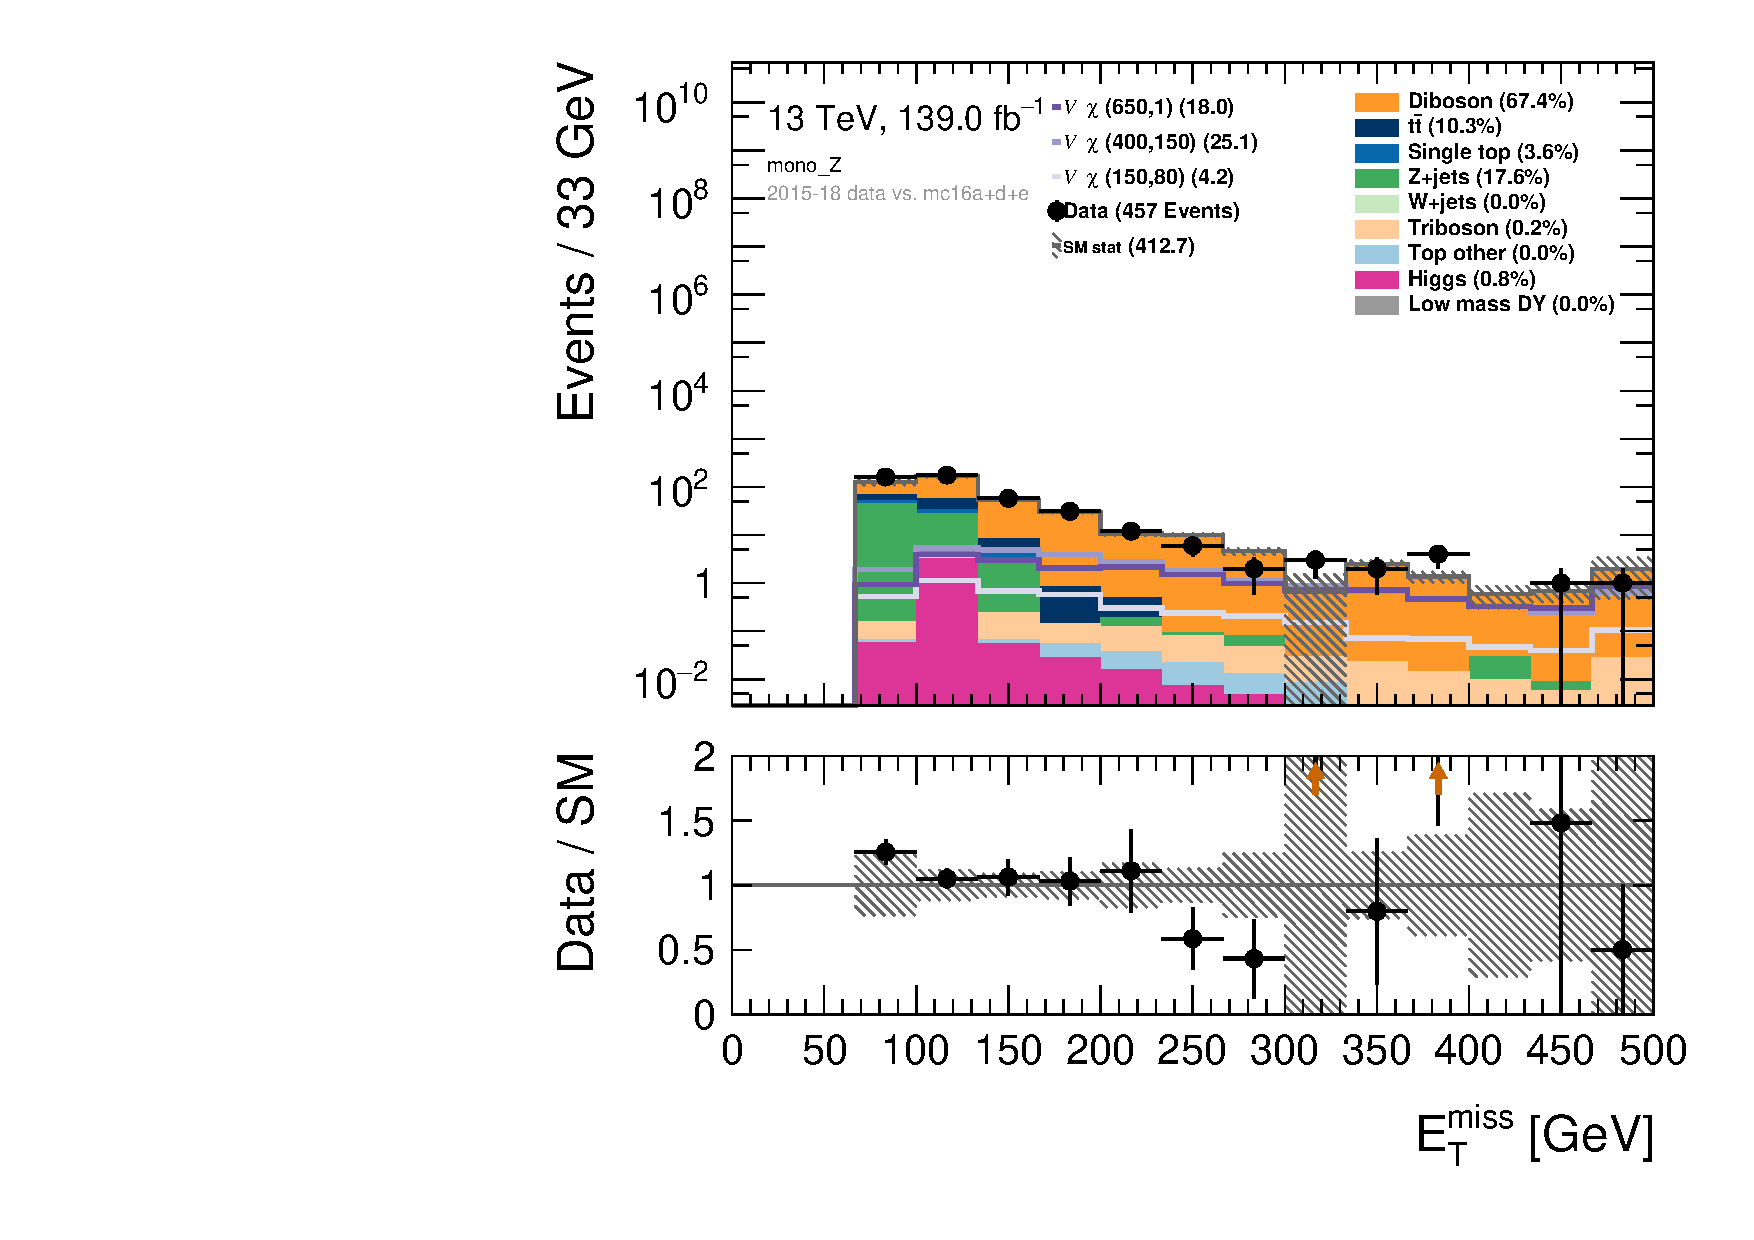
\includegraphics[width=\textwidth]{Figures/MonoZcuts/hist1d_met_Et_mono_Z.pdf}
    \caption{Stransverse mass for chargino production via $\Tilde{l}/\Tilde{\nu}$.}
    \label{fig:my_label}
    \end{subfigure}
    \caption{Plot of the four most important variables in direct slepton production with a cut on only two leptons with opposite charge in the final state.}
    \label{fig:cutandcountStepsDM}
\end{figure}
\restoregeometry